%One difficulty we have neglected so far is that 

%What we have available at this stage using 
The above procedure provides a precise mechanism to derive a statistic from the group-wise covariance matrix trajectories.
However, when the effect sizes are poor, any scheme operating on 
the trajectories of the {\em full covariance matrix} may still fail to identify group differences (as is the case in our experiments). To improve statistical power, localizing the process of computing the trajectories {\em 
  only to the relevant features} (subset selection) is critical. 
%Additionally, it serves as a discovery tool for exploratory analysis.
%
%
To this end, we consider the following global hypothesis testing problem
\begin{equation*}
H_0: \forall R, \Bbeta_1^R=\Bbeta_2^R \quad vs. \quad H_1: \exists R, \Bbeta_1^R\ne\Bbeta_2^R,
\end{equation*}       
where $\Bbeta$ denotes the slope and $R$ is the \textbf{region of the covariance matrix}
{\em which only includes the relevant features}, see Fig. \ref{fg:ball}.
It turns out that by adapting {\em Scan statistics} \citep{fan2012control, arias2011detection}, we will be able to exclude the effect of irrelevant regions of the covariance 
matrix in the calculated trajectories. 
By extending this concept to graphs, we obtain an algorithm to identify {\em subsets of features} of the covariance matrix which show group differences that 
are otherwise unidentifiable, in a statistically rigorous way. 
%Naively, exponentially many feature subsets $\mathcal{O}(2^p)$ need to be considered when localizing.  Under some mild conditions, extensions of ``scan statistics'' allow computationally tractable localization without compromising type II error.

\subsection{Scan Statistics}
Scan statistics are a valuable tool for structured multiple testing.
%Known in the engineering literature as “moving window analysis”, 
%The main idea is to instantiate o
In its simplest form, we can consider a setting where we place a window (or box) over a region $R$ in an image and calculate 
a local statistic $L_R$, e.g., an average or a response to a convolution filter. 
%a small window over the data, calculating some local statistic (number of events for a
%point pattern, perhaps, or average pixel value for an image) for each window. 
Then, the window can be raster scanned at various locations in the image ($\cR$) and the maximum 
over the set of local statistics is called the scan statistic. 
%The  
%The supremum
%or maximum of these locality statistics is known as the scan statistic, denoted M(X).
%Under
%some specified “homogeneity” null hypothesis H0 on X (Poisson point process, perhaps,
%or Gaussian random field) 
Intuitively, if the image is assumed to be a Gaussian random field, we can set up a null hypothesis using a
critical value and finding a statistically significant signal (i.e., regions) corresponds to comparing 
the local region-wise statistic with the critical value.  
%the approach entails specification of a critical value cα such that
%PH0 [M(X) ≥ cα] = α. If the maximum observed locality statistic is larger than or equal to
%cα, then the inference can be made that there exists a nonhomogeneity—a local region with
%statistically significant signal.
Of course, there is flexibility in terms of specifying properties of the regions as described next. 
 
\begin{definition} Let $\cR$ be the collection of all possible structured regions, and $L_R$ be some statistic over region $R$, a structured subset of $\cR$. The scan statistic is defined as $L^* = \max_{R\in\cR} L_R$.
\end{definition}
Recent results in scan statistics show how \textit{size corrections} can be used to increase detection power in multi-scale analysis with 
nice guarantees \citep{walther2010optimal,wang2016structured}. 
%With size corrections, scan statistics have been shown to be able to detect signal at level that theoretically no other detectors can improve \cite{walther2010optimal,wang2016structured}.
%
To utilize these ideas for our hypothesis test, we must extend scan statistics and these size corrections to a graph setting 
where the graph is induced by a sparse estimation of the precision matrix, e.g., graphical lasso (or any other algorithm of choice) over the features.
%, we can nicely define scan statistics on a graph.
%In order to define scan statistics on a graph, 
%effectively apply these methods, 
To do so, structured regions $R$ and a statistic $L_R$ on each region must be defined on the graph. Intuitively, in our case, 
$L_R$ must capture the ``difference'' in group-wise covariance trajectories. 
As we will describe shortly, it is in the context of this statistic where we utilize the LCGLM \eqref{eq:LCGLM}, which will be invoked at the {\em level of individual regions} $R$, one by one. 
%Since we have 
%In our setting, we can take advantage 
%a natural sparse graph structure which is estimated by graphical lasso in the previous section. 

Let $G:=(\cV,E)$ be a graph over the features (represented in the covariance matrix) with vertex set $\cV$ (to avoid overlap with tangent vectors) and edge set $E$. 
We define the structured region $R \subseteq G$ as a connected subgraph of $G$ corresponding to the 
selection of those vertices as our feature subset (block of the covariance matrix, see Fig. \ref{fg:ball}). 
A natural question is whether such an enumeration is tractable 
if the number of connected subgraphs $\cR$ is exponential. It turns out that if we make a mild assumption on the graph, 
the number of induced regions can be shown to be polynomially bounded. Further, it then naturally provides a {\em size correction}, the analog for a multiple testing adjustment. 

In our motivating application, the group differences we seek to identify will involve a cohesive set of features that will be 
connected to each other, by definition (large changes in covariances indicate dependent features). 
%features in one neighborhood are believed to behave similarly. 
Based on this observation, we assume that the true localized subgraph is a ``ball'' subgraph. 
\begin{definition} A ball subgraph consists of nodes with a given radius $r$ from a particular node (see Fig. \ref{fg:ball}). The collection of ball subgraphs is defined as
\begin{equation}
\cR=\left\{B(v,r):v\in \cV\ {\rm and}\ r\in \NN\right\}
\end{equation}
where the ball subgraph $B(v,r):=\{v^\prime \in \cV:d(v,v^\prime)\le r\}$, and $d(v,v^\prime)$ is the minimum length path connecting $v$ and $v^\prime$.
\end{definition}
%\textbf{Ball subgraph.} The collection of subgraphs of interest can be defined as $\cR=\left\{B(v,r):v\in \mV\ {\rm and}\ r\in \NN\right\}$,
%where the ball subgraph $B(v,r):=\{v^\prime \in V:d(v,v^\prime)\le r\}$, and $d(v,v^\prime)$ is the minimum length path connecting $v$ and $v^\prime$. 
%
With this assumption, it can be verified that we now only need to search a polynomially bounded set of regions.
\begin{remark}
The number of unique ball subgraphs in any graph $G$ is bounded above by $D|\cV|$, where $D$ is the diameter (longest chain) of the graph $G$.
\end{remark}
 On these regions 
(i.e., blocks of covariance matrix), 
we will invoke LCGLM to provide us a statistic $L_R$. This is just the difference in slopes of the calculated manifold regression across groups in \eqref{eq:traj}. 
We will iteratively obtain this statistic for distinct regions $R$ and find subgraphs that differ in their trajectories across groups using a size correction for hypothesis tests.
\begin{figure}
	\begin{center}
		%\scalebox{0.6}
		{
			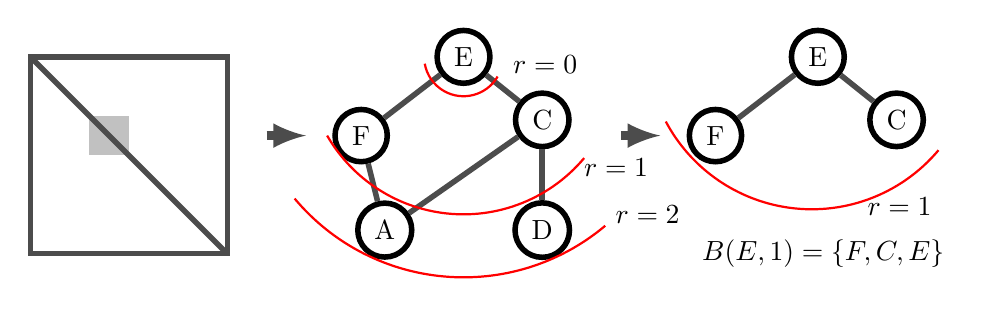
\begin{tikzpicture}
			\path[draw,line width=2pt,black!70!white] (-0.5,-0.5) -- (2,-0.5)--(2,2)--(-0.5,2)--cycle; 
			\fill[black!30!white,fill opacity=0.8] (0.75,0.75) -- (0.75,1.25) -- (0.25,1.25) -- (0.25,0.75) --cycle ; 
			\path[draw,line width=2pt,black!70!white] (-0.5,2)--(2,-0.5);
			
			\draw[-latex,thick,black!70!white,line width=3pt](2.5,1)
			to[out=0,in=180] (3.0,1);
			
			\node[shape=circle,draw=black,line width=2pt] (A) at (4,-0.2) {A};
			\node[shape=circle,draw=black,line width=2pt] (F) at (3.7,1) {F};
			\node[shape=circle,draw=black,line width=2pt] (C) at (6,1.2) {C};
			\node[shape=circle,draw=black,line width=2pt] (D) at (6,-0.2) {D};
			\node[shape=circle,draw=black,line width=2pt] (E) at (5,2) {E};
			\path [draw,line width=2pt,black!70!white] (A) edge node {}  (F);
			\path [draw,line width=2pt,black!70!white] (A) edge node {}  (C);
			\path [draw,line width=2pt,black!70!white] (E) edge node {}  (F);
			\path [draw,line width=2pt,black!70!white] (E) edge node {}  (C);
			\path [draw,line width=2pt,black!70!white] (C) edge node {}  (D);
			
			\draw[-latex,thick,black!70!white,line width=3pt](7.0,1)
			to[out=0,in=180] (7.5,1);
			
			\node[shape=circle,draw=black,line width=2pt] (B2) at (8.2,1) {F};
			\node[shape=circle,draw=black,line width=2pt] (C2) at (10.5,1.2) {C};
			\node[shape=circle,draw=black,line width=2pt] (E2) at (9.5,2) {E};
			\path [draw,line width=2pt,black!70!white] (E2) edge node {}  (B2);
			\path [draw,line width=2pt,black!70!white] (E2) edge node {}  (C2);
			
			\draw[thick,red] ([shift=(-40:2)]9.5,2.1) arc (-40:-152:2.1);
			\draw[thick,red] ([shift=(-40:2)]5,2) arc (-40:-150:2);
			\draw[thick,red] ([shift=(-30:0.5)]5,2) arc (-30:-170:0.5);
			\draw[thick,red] ([shift=(-50:2.8)]5,2) arc (-50:-140:2.8);
			
			\draw[thick,black](5.5,1.9)node[right]{$r=0$};
			\draw[thick,black](6.4,0.6)node[right]{$r=1$};
			\draw[thick,black](6.8,0)node[right]{$r=2$};
			%         \draw[thick,black](8.7,0.8)node[right]{$B(E,1)$};
			\draw[thick,black](10,0.1)node[right]{$r=1$};
			%\draw[thick,black](0.4,-1.3)node[right]{$(a)$};
			%\draw[thick,black](4.75,-1.3)node[right]{$(b)$};
			%\draw[thick,black](9.15,-1.3)node[right]{$(c)$};
			\draw[thick,black](7.9,-0.5)node[right]{$B(E,1)=\{F,C,E\}$};
			
			\end{tikzpicture}
		}
	\end{center}
	\caption[Covariance matrix regions and corresponding ball subgraphs]{\label{fg:ball} (left) A region of the sparse precision matrix, (center) The corresponding subgraph of that region, along with balls of varying radius from the root node $E$, (right) The ball subgraph constructed with $r = 1$.  These subgraphs with bounded radius act as the 
		structured regions on which scan statistics can be applied.}
\end{figure}
%To measure the change of dependence relationship between features, 
%we first fit a linear model for each element on covariance matrices over time for each group, i.e.,  $\beta_{g,ij} = \arg\min_{\alpha,\beta} \sum_{k=1}^T \|S_{k,g,ij} - \alpha - t_k\beta\|^2$, where $g$ is a group index $\{1,2\}$.
%the regression coefficient fit to the $i,j$-th position of the covariance matrices for both groups, i.e., $\beta_{g,ij} = \arg\min_{\alpha,\beta} \sum_{k=1}^T \|S_{k,g,ij} - \alpha - t_k\beta\|^2$. We call $B_g:=\beta_{g,ij}$ as a slop matrix.
%Now, we define a measurement, denoted by $X_e=|\beta_{1,ij} - \beta_{2,ij}|$, on each edge $e=(i,j)\in E$, indicating the correlation slope difference between feature $i$ and $j$.  To investigate the group effect within a subgraph $R$, it's straightforward to define a simple statistic as
%% \begin{align}
%% L_R = {\sum_{(i,j)\in E(R)}|\beta_{1,ij} - \beta_{2,ij}|\over \sqrt{|E(R)|}}
%% \end{align}
%where $E(R)$ represents all edges induced by subgraph $R$ and $|E(R)|$ is the number of edges in $E(R)$.
%To keep the variance of $L_R$ the same, we use $\sqrt{|E(R)|}$ instead of $|E(R)|$ in denominator of  $L_R$.
%Defined in this manner the calculation of this statistic is simple; we compute $L_{\cR}$ over all features, and then $L_R$ is simply the submatrix of $L_{\cR}$ indexed by the features $i,j \in R$.

Let us revisit the standard linear model setting and assume that 
our slopes $\Bbeta_g^R$ correspond to the subset of slopes from features in $R$, and $\hat{\Bbeta}_g^R$ is an estimate of that slope. In this case, we have the following  statistic (see e.g. \cite{seber2003linear}),
\begin{align}
(\hat{\Bbeta}_1^R - \hat{\Bbeta}_2^R)\Sigma_R^{-1}(\hat{\Bbeta}_1^R - \hat{\Bbeta}_2^R) \sim \chi_{|E(R)|}^2,
\end{align}
where $\Sigma_R^{-1}$ is the covariance matrix of $\hat{\Bbeta_1^R} - \hat{\Bbeta_2^R}$, and $E(R)$ denotes the number of edges among vertices in the subgraph $R$. With a normal noise assumption, this covariance will 
be identity and the statistic would simply be the $\ell_2$-norm difference as in the classical analysis. 
To make the statistics comparable across {\em different sizes}, we use the standardized version of a $\chi_{|E(R)|}^2$ distribution,
{\small\begin{align}\label{eq:LRstat}
L_R = \frac{(\hat{\Bbeta}_1^R - \hat{\Bbeta}_2^R)\Sigma_R^{-1}(\hat{\Bbeta}_1^R - \hat{\Bbeta}_2^R) - E(R) }{ \sqrt{E(R)} }.
\end{align}}
We can extend this analysis to our manifold setting.
\begin{definition}
For a given structured region $R$, the region-based LCGLM is written as
{ \begin{equation}
%\begin{split}
(b_g^R,\BV_g^R) = \arg\min_{(b^R,\BV^R) \in T\Mc^R} 
	\EE \left[ d(\EXP(b^R, \BV^R t_g),C_g^R)^2\right]
%\end{split}
\end{equation}}
where $C_g^R$ is the covariance matrix subblock defined by features included in $R$ for group $g$ ($t_g$ is our univariate predictor, i.e., time).
\end{definition}
\todo{ch3: fig: pt+stat pipeline}
To compare the group trajectories, we first parallel transport each tangent vector to the identity as described in \S\ref{sec:mglm} and then compute the statistic in \eqref{eq:traj} given as $\|\Gamma_{b_1^R \rightarrow I} \BV_1^R - \Gamma_{b_2^R \rightarrow I} \BV_2^R \|_{I}^2$.
In the case of the product space construction, we apply the test in \eqref{prop_prodstat} to the data subset corresponding to the features 
in region $R$, with the same correction as in \eqref{eq:LRstat}.

\paragraph{Summary.} We now have a region-based statistic for the manifold regression setting that is approximately normally distributed $N(0,1)$, allowing effective comparison across differently-sized regions.

%\iffalse
%{ \color{red}
%Now, given a structured region $R$, we can define $L_R$ using our statistic from Section \ref{sec:hyp-test}. The MMGLM defined for region $R$ can be written as
%\begin{equation*}
%\begin{split}
%(b_g^R,\BV_g^R) = \argmin_{(b^R,\BV^R) \in T\Mc^R} 
%	\EE \left[ d(\EXP(b^R, \BV^R t_g),C_g^R)^2\right]
%\end{split}
%\end{equation*}
%where $C_g^R$ is the subblock of the covariance matrix defined by the features included in $R$ for group $g$ and $t_g$ is our univariate predictor, time. With this estimate of the mean and tangent vector for both groups, the statistic is as in \eqref{eq:traj}, with a slight adjustment. If we normalize by the covariance of our estimate, this difference of slopes can be naturally interpreted as $\chi^2$ distributed with $E(R)$ degrees of freedom.{\color{blue}(If we don't introduce linear model and normal assumption, we can't say it follows the chi square distribution!!! We have to introduce linear model theory and say the manifold can borrow idea from there, otherwise the claim is wrong. We also need to distinguish the true value $\Bbeta^R$ and estimator $\hat{\Bbeta}^R$)} Let the vectorized ``slopes" for groups 1 and 2 be $\Bbeta_g^R = vec(\Gamma_{b_g^R \rightarrow I} \BV_g^R)$. {\color{blue}In linear model (see, e.g. \cite{seber2003linear})},  
%\begin{align}
%(\hat{\Bbeta}_1^R - \hat{\Bbeta}_2^R)\Sigma_R^{-1}(\hat{\Bbeta}_1^R - \hat{\Bbeta}_2^R) \sim \chi_{|R|}^2
%\end{align}
%{\color{blue}Here $\Sigma_R$ is the covariance matrix of $\hat{\Bbeta}_1^R - \hat{\Bbeta}_2^R$. To make statistics comparable across different sizes, we use the standardized version} of a $\chi_{|R|}^2$ distribution,
%{\begin{align}
%L_R = \frac{(\hat{\Bbeta}_1^R - \hat{\Bbeta}_2^R)\Sigma_R^{-1}(\hat{\Bbeta}_1^R - \hat{\Bbeta}_2^R) - E(R) }{ \sqrt{E(R)} }
%\end{align}
%}
%We have a region-based statistic that is approximately normally distributed $N(0,1)$.
%}
%\fi
\subsection{Size Correction}
%To improve detection power, 
A final unresolved yet important issue is that we must correct $L_R$ based on the number of edges $E(R)$ in $R$.
%Following the ideas of \cite{wang2016structured}, 
This has a direct consequence on detection power.
Observe that the normalization for size correction should be determined by the null distribution of $L_R$, i.e., 
when there is no slope difference in the trajectories between groups.
In order to derive a correction, we need to characterize the behavior of scan statistics within roughly similar regions, $\max_{R\in \cR(A)}L_R$, 
where $\cR(A)$ is the collection of region $R$s with similar size as $E(R)$,
\begin{align}
\cR(A)=\{R\in \cR:A/2<|E(R)|\le A\}.
\end{align}
Clearly, the behavior of $\max_{R\in \cR(A)}L_R$ depends on the ``complexity'' of $\cR(A)$. 
A clear understanding of how similar subgraphs relate to each other leads directly to a correction tied to their relative sizes.

To investigate the complexity of $\cR(A)$, we define the following quantities.
\begin{definition} The distance between subgraphs $R_1$ and $R_2$ can be given as
{\begin{align}
d(R_1,R_2)=1-\frac{|E(R_1)\cap E(R_2)|}{ \sqrt{|E(R_1)||E(R_2)|}}
\end{align}}
\end{definition}
\begin{definition}
Let the $\epsilon$-covering number of $\cR(A)$, denoted by $N(A,\epsilon)$, be the smallest integer such that there
is a subset $\cR_{approx}(A,\epsilon)$ of $\cR$ such that
{\begin{align}
\sup_{R_{1}\in\cR(A)}\inf_{R_{2}\in \cR_{approx}(A,\epsilon)}d(R_{1},R_{2})\le \epsilon
\end{align}}
where $|\cR_{approx}(A,\epsilon)|=N(A,\epsilon)$.
\end{definition}
We can verify that all regions in $\cR(A)$
can be approximated by regions in $\cR_{approx}(A)$ with reasonably small error.
From the definitions, notice that the complexity of $\cR(A)$ is reflected by $N(A,\epsilon)$.
If $N(A,\epsilon)$ is nicely bounded (as is the case here), scan statistics can be calculated very efficiently 
(Lemma \ref{lm:entropy}). 
%, as presented 
%shortly in Lemma \ref{lm:entropy}.
%For more details and intuition, please refer to \cite{wang2016structured}.

Before stating this result, we make a mild assumption on our graph. 
For any ball subgraph, the edges around its center are not too sparse, compared to the edges 
in the outer region of the ball subgraph, i.e., hard on the inside, soft on the outside. This yields, 
\begin{assumption}(Avocado) There exist constants $S$ and $H$ such that, for any $r/2 \leq r' \leq r$ and $v \in \cV$,
{\begin{align}\label{eq:lightskirt}
\frac{|E(B(v,r'))|}{|E(B(v,r))|} \geq H\left(1 - \frac{|E(B(v,r-r'))|}{|E(B(v,r))|}\right)^S.
\end{align}}
\end{assumption}
We see that this assumption holds for many classes of graphs:
a ring graph satisfies this condition when $H=1$ and $S=1$ and the 2-D lattice satisfies this condition when $H=1/4$ and $S=2$ (see Fig. \ref{fg:avocado}). 
\begin{figure}
	\begin{center}
		\scalebox{0.8}
		{
			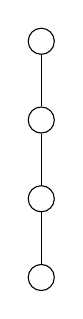
\begin{tikzpicture}
			\tikzstyle{vertex}=[circle,draw,minimum size=0.2cm]
			\tikzstyle{every node}=[vertex]
			
			\node (A) { };
			\node (B) [below of = A] { };
			\node (C) [below of = B] { };
			\node (D) [below of = C] { };
			\draw (A) -- (B);
			\draw (B) -- (C);
			\draw (C) -- (D);
			
			
			\end{tikzpicture}
			\hspace{0.2cm}
			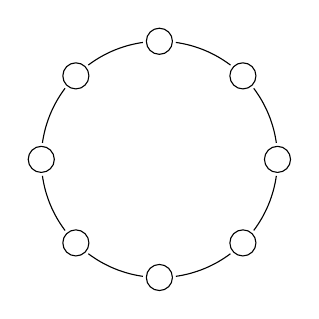
\begin{tikzpicture}
			\def \n {8}
			\def \radius {1.5cm}
			\def \margin {8} % margin in angles, depends on the radius
			
			\foreach \s in {1,...,\n}
			{
				\node[draw, circle] at ({360/\n * (\s - 1)}:\radius) { };
				\draw[-, >=latex] ({360/\n * (\s - 1)+\margin}:\radius) 
				arc ({360/\n * (\s - 1)+\margin}:{360/\n * (\s)-\margin}:\radius);
			}
			\end{tikzpicture}
			\hspace{0.2cm}
			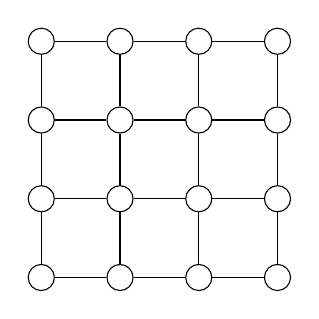
\begin{tikzpicture}%[circle, draw, minimum size=1cm, every node=[vertex]]
			\tikzstyle{vertex}=[circle,draw,minimum size=0.2cm]
			\tikzstyle{every node}=[vertex]
			\foreach \x in {1,2,3,4}
			{
				\foreach \y in {1,2,3,4}
				{
					\node (\x \y) at (\x,\y) { };
					\ifnum\y>1
					\pgfmathparse{int(\y-1)}  
					\draw  (\x \y)  -- (\x \pgfmathresult);
					\fi
					\ifnum\x>1
					\pgfmathparse{int(\x-1)}                
					\draw (\x \y) -- (\pgfmathresult \y);
					\fi 
				}
			}   
			\end{tikzpicture}
			\hspace{1cm}
			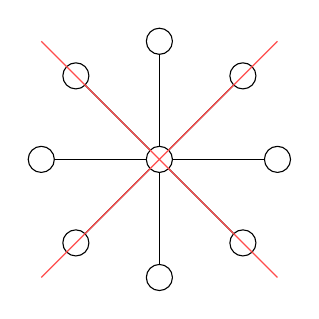
\begin{tikzpicture}
			\def \n {8}
			\def \radius {1.5cm}
			
			\node[draw, circle] (ss) at ({0}:0) { };
			
			\foreach \s in {1,...,\n}
			{
				\node[draw, circle] (\s) at ({360/\n * (\s - 1)}:\radius) { };
				\path (ss) edge [] node { } (\s);
			}
			\path[draw,line width=0.5pt,red!70!white] (-1.5,1.5)--(1.5,-1.5);
			\path[draw,line width=0.5pt,red!70!white] (-1.5,-1.5)--(1.5,1.5);
			\end{tikzpicture}
		}
	\end{center}
	\caption[Avocado graphs]{\label{fg:avocado} (Left) Chain, ring and 2D lattice graphs that satisfy the Avocado Assumption. (Right) Star graph that does not satisfy the property: from the center node the graph is ``too dense on the outside."}
\end{figure}
With this assumption, we have the following result for the $\epsilon$-covering number $N(A,\epsilon)$.
\begin{lemma}
	\label{lm:entropy}
        Let $|E|$ be the total number of edges in $G$. If (\ref{eq:lightskirt}) holds and $A$ is given, 
        then, for a constant $C_{H,S}$ which only depends on $H$ and $S$ in (\ref{eq:lightskirt}),
	{\begin{equation}
	    \label{eq:entropy}
	    N(A,\epsilon)\le C_{H,S}\frac{|E|}{ A}\left(\frac{1}{ \epsilon}\right)^{S+1}.
	\end{equation}}
\end{lemma}
The proof of this result follows from our ball-subgraph construction and our Avocado assumption and is provided in the Appendix.

Intuitively, this result upper bounds the number of graphs that are necessary to search over to completely exhaust the search space of subgraphs. With this result, we can now construct a suitable size correction. 
Following the work of \cite{walther2010optimal} and \cite{wang2016structured}, we can increase the power of our test by using the following statistic:
% when there's no correlation slope difference across groups. 
%To simplify the analysis, we assume null distribution of each $L_R$ follows normal distribution with mean $0$ and variance $1$ at this moment. This assumption generally holds when tangent normal noise assumption.
%And we also assume $L_{R_1}-L_{R_2}$ follows normal distribution with mean $0$ and variance $C'd(R_1,R_2)$ for some constant $C'$. 
%The intuition behind this assumption is that $L_{R_1}$ should behave very similar with $L_{R_2}$ when $R_1$ and $R_2$ has large overlapping region(i.e. $d(R_1,R_2)$ is small).
%Although this assumption does not always hold, this can guide us to obtain the suitable form of size correction.
%With these assumptions, we can actually obtain following theorem:
% \begin{theorem}
% If $X_e$ follows independent normal distribution $N(0,1)$ and (\ref{eq:entropy}) holds, then, for all $t>1$,
% \begin{align*}
% \PP\left(\max_{R\in \cR(A)}L_R> \sqrt{2\log{|E|\over A}}+t\right)\le C_1\exp\left(-C_2t^2\right) 
% \end{align*}
% for some constant $C_1$ and $C_2$.
% \end{theorem}
%Motivated by this result, the suitable way to do size correction is to subtract $\sqrt{2\log{|E|/|E(R)|}}$ from each $L_R$. 
%Therefore, we propose the following this size corrected scan statistic:
{\begin{align} \label{eq:scanstat}
T^\ast=\max_{R\in\cR}\left(L_R-2\sqrt{\log\frac{|E|}{ |E(R)|}}\right).
\end{align}}
%This result requires that the measures over each region that define $L_R$ are defined on each edge $E(R)$. In our particular construction, the statistic $L_R$ is defined as a function a complete measure of the difference of the tangent vectors. Therefore, we can define our \textit{manifold-valued size corrected scan statistic} as:
%{\begin{align} \label{eq:manscanstat}
%T^\ast=\max_{R\in\cR}\left(L_R-\sqrt{2\log\frac{|\text{dim}(\Mc)|}{ |\text{dim}(\Mc^R)|}}\right).
%\end{align}}
The significance of this size correction is that we now have \textit{a single critical value for each candidate subgraph, regardless of the subgraph size}. Our final test is defined as $\mathbb{I}[T^* > q_\alpha]$, where $q_\alpha$ is the $\alpha$-level quantile of $T^*$ under the null hypothesis (that no region is truly significant across groups). By construction, we can control the type 1 error at a specified $\alpha$-level.

Under the alternative hypothesis of this framework, it is important to note that in many cases,
large subgraphs that subsume smaller significant graphs may also have large test statistics, and our hypothesis test only indicates the existence of {\em some} significant region. To identify or localize the smaller subsets, we follow the procedure from \cite{jeng2010optimal}, by beginning with the subgraph with the largest test statistic and iteratively removing overlapping subsets from the total set of subgraphs. This requires testing each regional/local statistic, $(L_R - 2\sqrt{\log(|E|/|E(R)|)})$ against $q_\alpha$. Under this procedure, we can control the weak family-wise error rate (wFWER) if we view our problem via the lens of multiple testing. The weak FWER is the probability of false discovery under the null hypothesis. To see that this is inherently controlled, note
\begin{align}
\mathbb{P}(FN \geq 1|H_0) = \mathbb{P}(T^* > q_\alpha|H_0) \leq \alpha, 
\end{align}
where $FN$ is the number of false discoveries under the null hypothesis. With this correction at the group difference level, we completely avoid any multiple comparisons issues that would arise in the case of a test for each subgraph.
%
In addition to controlling the false positive rate, we have the following guarantee on {\em identifying truly significant regions} under the normal noise assumption.
\begin{theorem}
If \eqref{eq:lightskirt} holds and the number of edges in the candidate subgraph is larger than $\log^2 |E|$, i.e.,
\begin{equation}
\label{eq:setsize}
|E(R)|\gg \log^2 |E|\qquad \forall\ R\in\cR,
\end{equation}
then the critical value $q_\alpha$ satisfies
\begin{equation}
\label{eq:criticalvl}
q_\alpha=O(1).
\end{equation}
Moreover, as $|E|\to \infty$, if a subgraph $R_0$ obeys 
\begin{equation}
\label{eq:sigcond}
\frac{(\Bbeta_1^{R_0}-\Bbeta_2^{R_0})^T\Sigma_{R_0}^{-1}(\Bbeta_1^{R_0}-\Bbeta_2^{R_0})}{\sqrt{|E({R_0})|}}\gg 2\sqrt{\log\frac{|E|}{|E({R_0})|}},
\end{equation}
then as $|E|\to \infty$,
\begin{equation}
\label{eq:power}
\PP\left(L_{R_0}-2\sqrt{\log\frac{|E|}{|E({R_0})|}}>q_\alpha\right)\to 1.
\end{equation}
\label{lm:mainthm}
\end{theorem}
The full proof of this result follows a generic chaining argument (see, e.g. \cite{talagrand2006generic}) along with application of 
concentration inequalities and union bounds, and can be found in the Appendix. \todo{ch3: FWER proof appendix reference}

\paragraph{Summary.} At a high level, this result directly characterizes the behavior of $T^*$ under the null hypothesis $H_0$ and 
the alternative hypothesis $H_1$, respectively. 
We see that \eqref{eq:criticalvl} implies that $T^*$ can roughly be seen as a constant under the null hypothesis, 
and under the alternative hypothesis when \eqref{eq:sigcond} is satisfied, the test based on $T^*$ is consistent, see \eqref{eq:power}. 

\subsection{Workflow for conducting hypothesis tests on temporal trends of graphs}
\todo{ch3: fig: from presentation, full workflow}
%{\color{red} maybe refer to the video again?}{\color{blue} I think a flow chart of how the whole algorithm work may be helpful. Otherwise, it's difficult for audiences to get the idea if we only mention the test statistics and Jeng's paper.}
With these guarantees, our full workflow is as follows. First, we use an oracle procedure to generate a graph over our features 
that roughly captures the conditional independences. Any procedure that provides a conditional independence graph is sufficient. 
Next, for each ball subgraph over this graph, we compute the Longitudinal-Covariance GLM over these features for both groups, and compute the statistics outlined in Section \ref{sec:hyp-test}. We then compute the size-corrected statistic, and compare against the single critical value. For all regions that pass this threshold, we apply the procedure from \cite{jeng2010optimal}. This workflow shows how to conduct hypothesis tests on temporal trends of large covariance matrices, with improved 
power and bounded Type 1 error. Additional implementation details can be found in the Appendix.
